\section{Geometry of representations learned by MD-IPR and Relational Convolutions}\label{sec:appendix_rep_analysis}

In this section, we explore and visualize the representations learned by MD-IPR and RelConv layers. In particular, we will visualize the representations produced by the RelConvNet model trained on the \textit{Set} task described in~\Cref{ssec:experiments_set}. Recall that the MD-IPR layer learns encoders $\phi_1, \psi_1, \ldots, \phi_{d_r}, \psi_{d_r}$. In this model $d_r = 16$, $\phi_i = \psi_i$ (so that learned relations are symmetric), and each $\phi_i$ is a linear transformation to $d_{\mathrm{proj}} = 4$-dimensional space. The representations learned by a selection of 6 encoders is visualized in~\Cref{fig:mdirp_encoders_rep}. For each of the 81 possible \textit{Set} cards, we apply each encoder in the MD-IPR layer, reduce to 2-dimensions via PCA, and visualize how each encoder separates the 4 attributes: number, color, fill, and shape. Observe, for example, that ``Encoder 0'' disentangles color and shape, ``Encoder 2'' disentangles fill, and ``Encoder 3'' disentangles number.

Next, we visualize, we explore the geometry of learned representations of relation vectors. That is, the inner products producing the 16-dimensional relation vector for each pair of objects. For each $\binom{81}{2}$ pairs of \textit{Set} cards, we compute the 16-dimensional relation vector learned by the MD-IPR layer, reduce to 2 dimensions via PCA, and visualize how the learned relation disentangles the latent same/different relations among the four attributes. This is shown in~\Cref{fig:mdipr_rel_rep}. We see some separation of the underlying same/different relations among the four attributes, even with only two dimensions out of 16.

Finally, we visualize the representations learned by the relational convolution layer. Recall that this layer learns a set of graphlet filters $\bm{f} \in \reals^{s \times s \times d_r \times n_f}$ which form templates of relational patterns against which groups of objects are compared. In our experiments, the filter size is $s = 3$ and the number of filters is $n_f = 16$. Hence, for each group $g$ of 3 \textit{Set} cards, the relational convolution layer produces a 16-dimensional vector, $\reliprod{R[g]}{\bm{f}} \in \reals^{n_f}$, summarizing the relational structure of the group. Of the $\binom{81}{3}$ possible triplets of \textit{Set} cards, we create a balanced sample of ``sets'' and ``non-sets''. We then compute $\reliprod{R[g]}{\bm{f}}$ and reduce to 2 dimensions via PCA.~\Cref{fig:conv_rep} strikingly shows that the representations learned by the relational convolution layer very clearly separate triplets of cards which form a set from those that don't form a set.


\begin{figure}
    \centering
    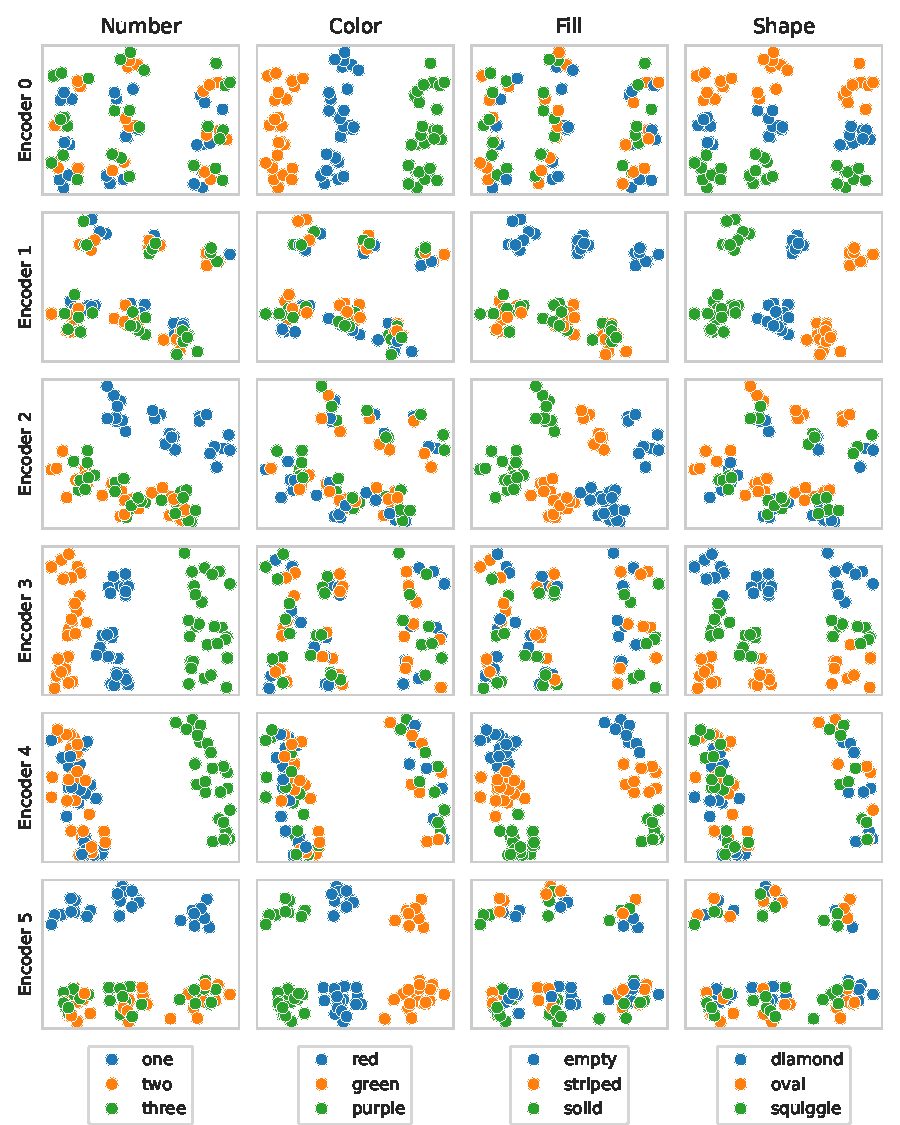
\includegraphics[width=0.9\textwidth]{figs/representation_analysis/mdipr_encoders_rep.pdf}
    \caption{The encoders learned in the MD-IPR layer represent the latent attributes in the \textit{Set} cards, with different encoders seemingly specializing to encode one or two attributes.}\label{fig:mdirp_encoders_rep}
\end{figure}

\begin{figure}
    \centering
    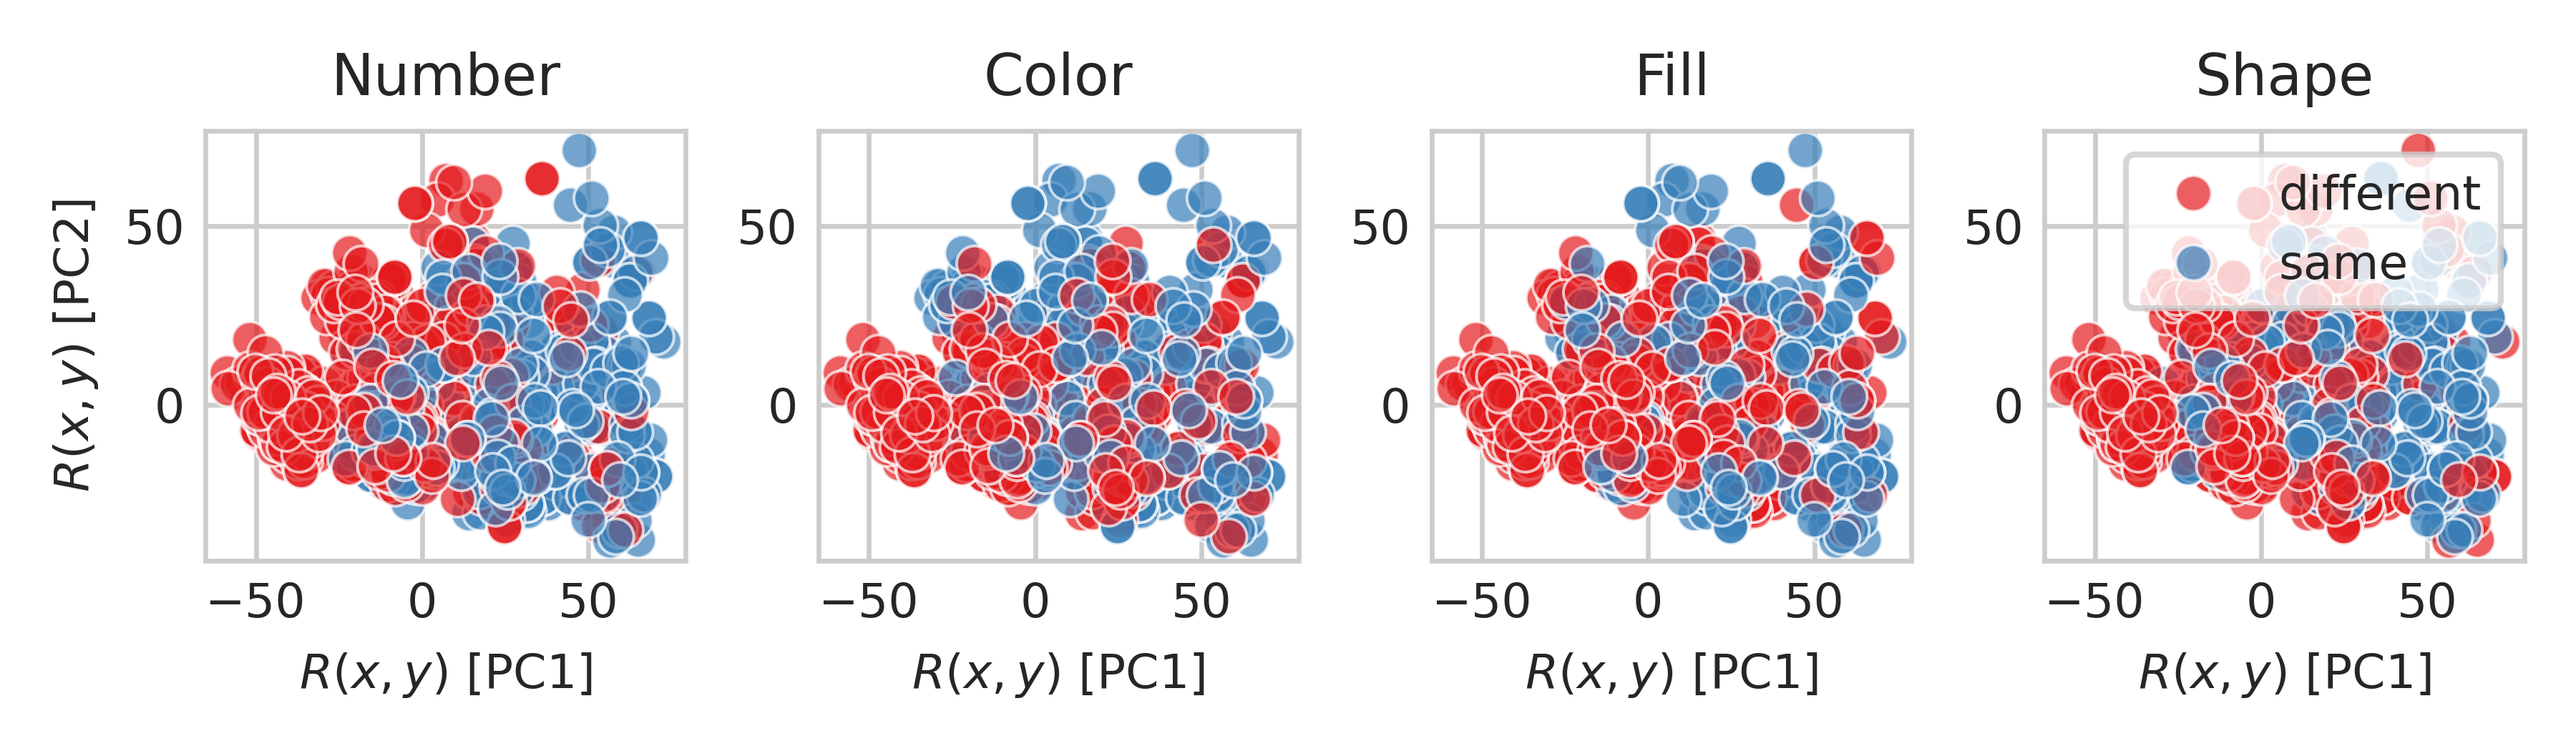
\includegraphics[width=0.95\textwidth]{figs/representation_analysis/mdipr_rel_rep.png}
    \caption{The relations learned by the MD-IPR layer encodes the latent relations underlying the \textit{Set} task.}\label{fig:mdipr_rel_rep}
\end{figure}

\begin{figure}
    \centering
    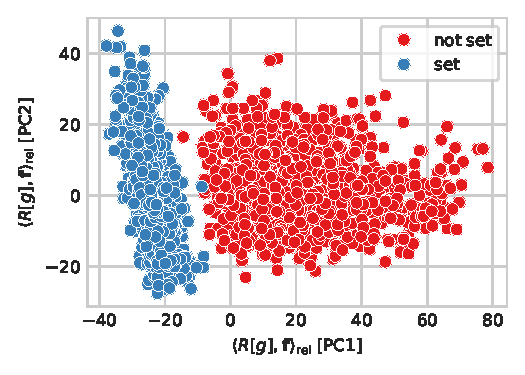
\includegraphics{figs/representation_analysis/conv_rep.pdf}
    \caption{The relational convolution layer produces representations which separates `sets' from `non-sets'.}\label{fig:conv_rep_appdx}
\end{figure}

% \null
% \vfill
